\subsection{Configuracion}
	Para poder correr el controlador y la topologia debemos abrir la maquina virtual. Luego abrir dos terminales como se explico en la 		seccion de maquina virual en desarrollo. Pra resumirlo en pasos, debemos:
	\begin{enumerate}
		\item Pararse en la raiz del repositorio
		\item abrir una terminal y ejecutar: $sh \; scripts/resync.sh$
		\item Luego, en la misma terminal ejecutar: $sh scripts/conect\_to\_VM.sh$. Nos pedira nuestra contraseña y la contraseña de la 		VM que es: $frenetic$
		\item Correr el controlador ejecutando: $pox/pox.py \; launch$
		\item Repetir el paso 3 en otra terminal.
		\item Levantar la topologia ejecutando: $sh \; Datacenter/scripts/lift\_topology.sh$
	\end{enumerate} 
\subsection{Pingall}
	Una vez que levantamos primero el controlador y luego la topologia, los sitches tienen su tabla vacia, por lo que el primer pingall 		sera consultado compeltamente al controlador para que resuelva las salidas. Por lo tanto el primer pingall siempre tardara un poco mas, 	y en algunos caso, algun ping puede llegar a perderse por un timeout. A continuacion mostramos un pingall apenas se levanto 
	la topologia y el controlador y otro pingall justo despues asi contrarestamos el tiempo que tardo cada uno:
	\begin{figure}[ht]
		\begin{adjustbox}{addcode={
			\begin{minipage}{\width}}{
				\caption{%
					Pingall apenas se levanto el controlador y la topologia
					}
			\end{minipage}},rotate=360,center}
			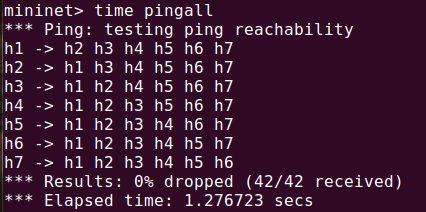
\includegraphics[scale=.6]{pics/pingall_1.png}
		\end{adjustbox}
	\end{figure}
	\FloatBarrier
	\begin{figure}[ht]
		\begin{adjustbox}{addcode={
			\begin{minipage}{\width}}{
				\caption{%
					Segundo Pingall
					}
			\end{minipage}},rotate=360,center}
			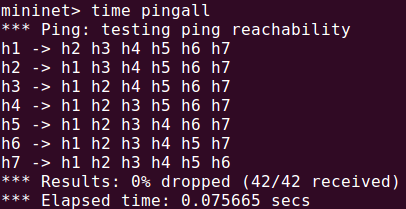
\includegraphics[scale=.6]{pics/pingall_2.png}
		\end{adjustbox}
	\end{figure}
	\FloatBarrier
	Podemos observar que no hubo perdidas, y ademas se ve claramente la diferencia de tiempo en que se resolvio los pings en cada caso 		donde en el primer caso se tardo unos $1.276723 \; segundos$ y en el segundo caso el tiempo disminuyo drasticamente 
	a unos $0.075665 \; segundos$.
\subsection{Balanceo de cargas con conexion TCP}
	Para realizar esta prueba vamos a utilizar la herrmienta $iperf$ para hacer una conexxion cliente-servidor entre dos hosts. Primero, 		vamos a ir a la terminal donde esta correindo mininet (donde levatamos la topologia) y en el prompt de mininet escribiremos 
	$xterm h1 h4$ para abrir dos terminales en cada host.\\
	Luego vamos a abrir otra terminal (conectada a la VM como se exlico antes) y escribiremos: $sudo wireshark \&$. Y abriremos la interfaz 		$s2-eth1$. Y abriremos otro wireshark de la misma manera, pero en la interfaz $s3-eth1$.\\
	Luego en la terminal del host 4 levantaremos el servidor escribriendo lo siguiente: $iperf \; -s \; -p \; 80$. En la terminal del 
	host 1 escribiremos lo sigueinte para hacer la conexion: $iperf \; -c \; 10.0.0.4 \; -p \; 80$. y lo que haremos es ver ambas ventanas 		de wireshark y comprobar que los paquetes TCP solo pasan por algunas de las dos interfaz, pero no en ambas.\\
	A continuacion mostramos la captura de las terminales en cada host. y la comprobacion del balanceo de cargas en wireshark:\\
	\begin{figure}[ht]
		\begin{adjustbox}{addcode={
			\begin{minipage}{\width}}{
				\caption{%
					Conexion TCP cliente host 1
					}
			\end{minipage}},rotate=360,center}
			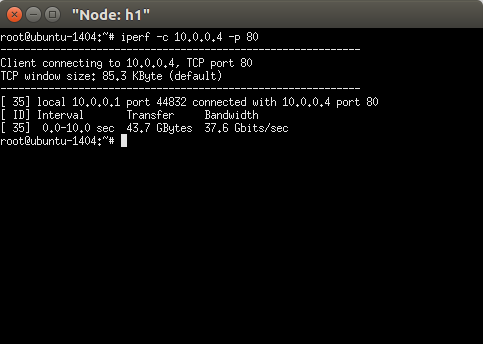
\includegraphics[scale=.6]{pics/iperf-h1-tcp.png}
		\end{adjustbox}
	\end{figure}
	\FloatBarrier
	\begin{figure}[ht]
		\begin{adjustbox}{addcode={
			\begin{minipage}{\width}}{
				\caption{%
					Conexion TCP servidor host 4
					}
			\end{minipage}},rotate=360,center}
			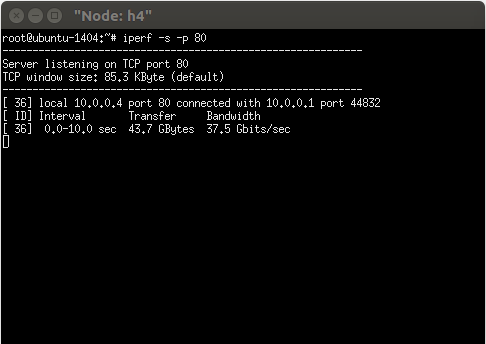
\includegraphics[scale=.6]{pics/iperf-h4-tcp.png}
		\end{adjustbox}
	\end{figure}
	\FloatBarrier
	Podemos comprobar que cumple con el balanceo de cargas ya que los paquetes solo viajan por el switch 2. Esto es asi, porque ir por 		cualquiera de los swtich es lo mismo respecto a llegar a desrino y a cuanto pesa el mismo, es decir, tenemos un empate y vemos que el 		controlador decidio que de acuerdo a este flujo se elija solo el switch 2:\\
	\begin{figure}[ht]
		\begin{adjustbox}{addcode={
			\begin{minipage}{\width}}{
				\caption{%
					Captura de wireshark monitoreando la interfaz eth1 del switch s2
					}
			\end{minipage}},rotate=360,center}
			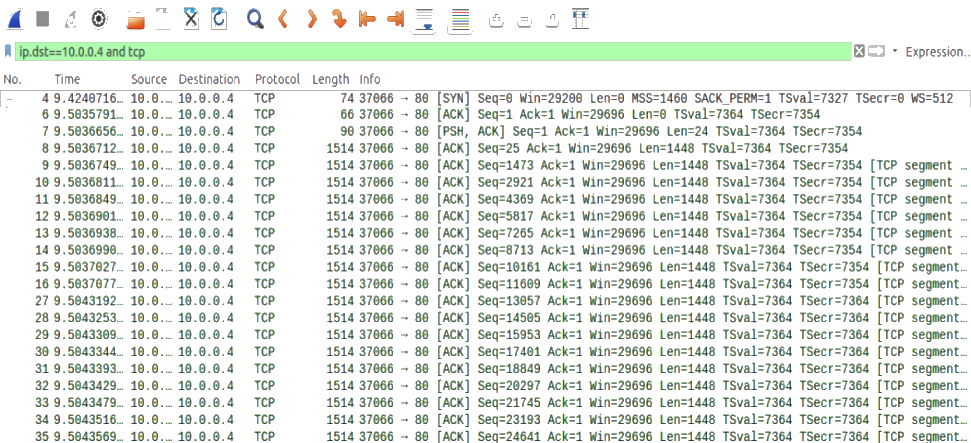
\includegraphics[scale=.6]{pics/s2-eth1-tcp-h1-h4.png}
		\end{adjustbox}
	\end{figure}
	\FloatBarrier
	\begin{figure}[ht]
		\begin{adjustbox}{addcode={
			\begin{minipage}{\width}}{
				\caption{%
					Captura de wireshark monitoreando la interfaz eth1 del switch s3
					}
			\end{minipage}},rotate=360,center}
			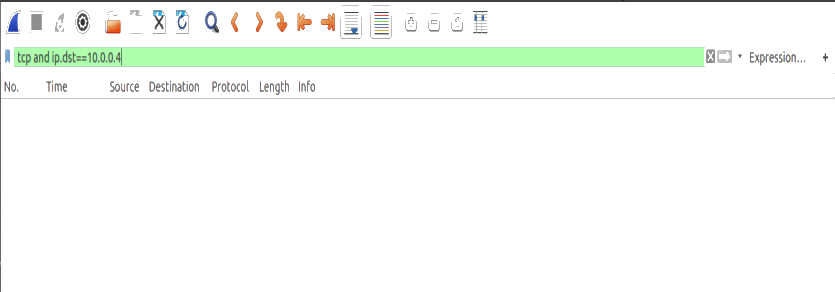
\includegraphics[scale=.6]{pics/s3-eth1-tcp-h1-h4.png}
		\end{adjustbox}
	\end{figure}
	\FloatBarrier

\subsection{Balanceo de cargas con ping}
	Para realizar esta prueba vamos a usar miniet haciendo un ping entre h1 y h5, y otro ping entre h2 y h5. De esta manera podremos ver 		que lo que deberia pasar es que un flujo deberia elegir el switch 2 o 3 y el otro flujo tambien sin que ambos elijan el mismo flujo. 		Los paquetes que se envian contienen un protocolo ICMP, por lo tanto haremos un monitoreo en la interfaces s3-eth1 y s2-eth1 para 		verificar que cuando hacemos el ping ehtre h1 y h5 una de ellas esta vacia y la otra recibe los paquetes, pero al hacer el ping entre 		h2 y h5 debemos poder ver los mismo pero en los switches invertidos.\\
	Primero mostramos el monitoreo en wireshark cuando hacemos el ping entre h1 y h5:\\
	\begin{figure}[ht]
		\begin{adjustbox}{addcode={
			\begin{minipage}{\width}}{
				\caption{%
					Captura de wireshark monitoreando la interfaz eth1 del switch s2
					}
			\end{minipage}},rotate=360,center}
			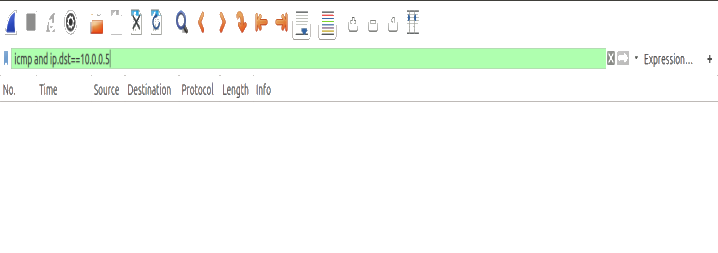
\includegraphics[scale=.6]{pics/s2-eth1-h1-ping-h5.png}
		\end{adjustbox}
	\end{figure}
	\FloatBarrier
	\begin{figure}[ht]
		\begin{adjustbox}{addcode={
			\begin{minipage}{\width}}{
				\caption{%
					Captura de wireshark monitoreando la interfaz eth1 del switch s3
					}
			\end{minipage}},rotate=360,center}
			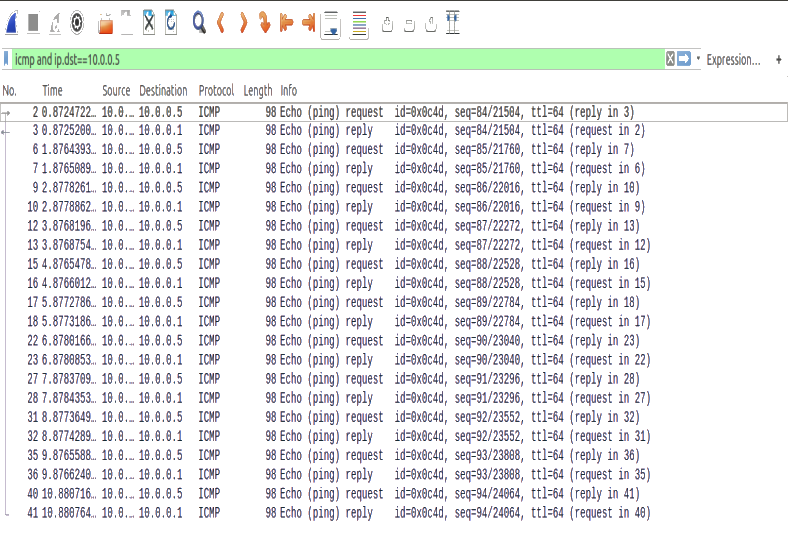
\includegraphics[scale=.6]{pics/s3-eth1-h1-ping-h5.png}
		\end{adjustbox}
	\end{figure}
	\FloatBarrier
	Luego mostramos el monitoreo en wireshark cuando hacemos el ping entre h2 y h5:\\
	\begin{figure}[ht]
		\begin{adjustbox}{addcode={
			\begin{minipage}{\width}}{
				\caption{%
					Captura de wireshark monitoreando la interfaz eth1 del switch s2
					}
			\end{minipage}},rotate=360,center}
			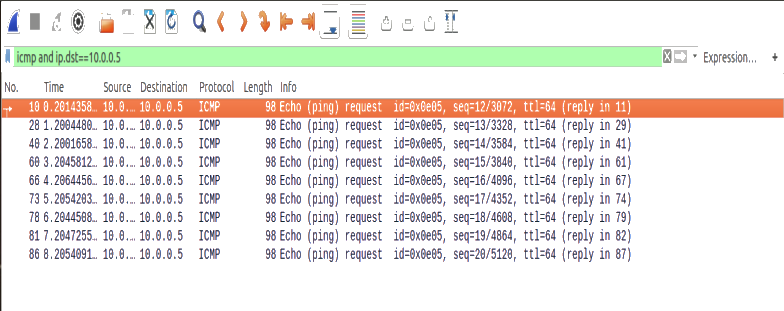
\includegraphics[scale=.6]{pics/s2-eth1-h2-ping-h5.png}
		\end{adjustbox}
	\end{figure}
	\FloatBarrier
	\begin{figure}[ht]
		\begin{adjustbox}{addcode={
			\begin{minipage}{\width}}{
				\caption{%
					Captura de wireshark monitoreando la interfaz eth1 del switch s3
					}
			\end{minipage}},rotate=360,center}
			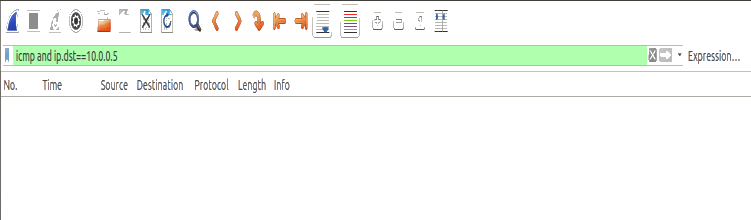
\includegraphics[scale=.6]{pics/s3-eth1-h2-ping-h5.png}
		\end{adjustbox}
	\end{figure}
	\FloatBarrier
	Como se puede observar, el ping entre h1 y h5 solo pasa por el switch 3 y el ping entre h2 y h5 solo pasa por el swtich 2.

\subsection{Denegacion de servicio}
	Para realizar esta prueba vamos a utilizar la herrmienta $iperf$ para hacer una conexxion cliente-servidor entre dos hosts. Primero, 		vamos a ir a la terminal donde esta correindo mininet (donde levatamos la topologia) y en el prompt de mininet escribiremos 
	$xterm h1 h5$ para abrir dos terminales en cada host.\\
	Luego vamos a abrir otra terminal (conectada a la VM como se exlico antes) y escribiremos: $sudo wireshark \&$. Y abriremos la interfaz 	$s5-eth1$.
	Luego en la terminal del host 5 levantaremos el servidor escribriendo lo siguiente: $iperf \; -u \; -s \; -p \; 80$. En la terminal del 
	host 1 escribiremos lo sigueinte para hacer la conexion: $iperf \; -u \; -c \; 10.0.0.4 \; -p \; 80$. y lo que haremos es ver ambas 		ventanas de wireshark y comprobar que los paquetes TCP solo pasan por algunas de las dos interfaz, pero no en ambas.\\
	A continuacion mostramos la captura de las terminales en cada host y la captura de wireshark y debemos comprobar que el host 1 devuelve 	un warning el cual dice que no se pudieron enviar todos los datagramas y por lo tanto en wireshar debemos poder recibir una cantidad 		menor a la que se queria enviar.\\
	\begin{figure}[ht]
		\begin{adjustbox}{addcode={
			\begin{minipage}{\width}}{
				\caption{%
					Conexion UDP servidor host 1
					}
			\end{minipage}},rotate=360,center}
			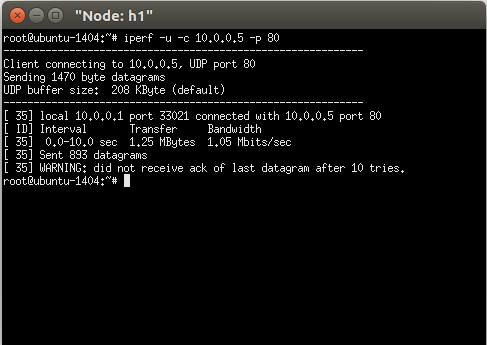
\includegraphics[scale=.6]{pics/iperf-h1-udp.png}
		\end{adjustbox}
	\end{figure}
	\FloatBarrier
	\begin{figure}[ht]
		\begin{adjustbox}{addcode={
			\begin{minipage}{\width}}{
				\caption{%
					Conexion UDP servidor host 5
					}
			\end{minipage}},rotate=360,center}
			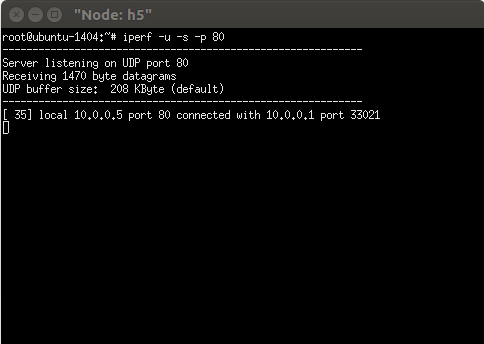
\includegraphics[scale=.6]{pics/iperf-h5-udp.png}
		\end{adjustbox}
	\end{figure}
	\FloatBarrier
	\begin{figure}[ht]
		\begin{adjustbox}{addcode={
			\begin{minipage}{\width}}{
				\caption{%
					Captura de wireshark monitoreando la interfaz eth1 del switch s5
					}
			\end{minipage}},rotate=360,center}
			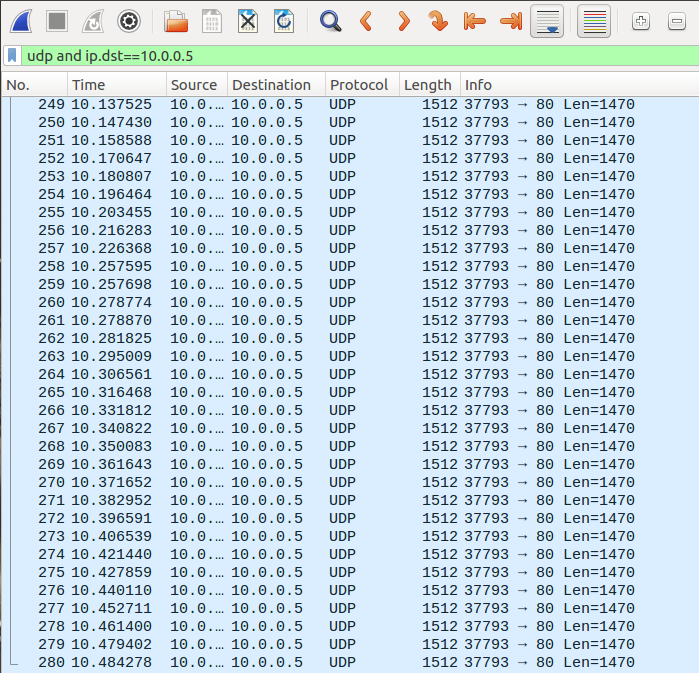
\includegraphics[scale=.6]{pics/s5-eth1-udp.png}
		\end{adjustbox}
	\end{figure}
	\FloatBarrier
	Como se puede observar, vemos que recibimos menos datagramas porque como dice en la temrinal del host 1, se quisieron enviar 893 y 		recibimos 280.
\subsection{Pruebas automaticas}
	Esta seccion se realizo a medias ya que en principio se realizaron test unitarion usando $pytest$ donde mediante wireshark, se lee la 		captura que se hizo con wireshark y se comprueba lo que se mostro anteriormente. Pero queda a modo de tareas a realizar poder ejecutar 		desde un solo script codigo que levante todas las terminales que hacen falta para podera hacer la concexion y mediante tcpdump, generar 	la capruta deseada. De esta manera, nuestros test no cambiarian, y siempre leerian un archivo $*.pcap$, donde mediante tshark se lo 		transforma en un txt para poder leerlo usando uan herramienta llamada $pandas$. En un futuro, como segundo release, se podria llevar a 		cabo dichos test y de esa manera de automatiza todo el proyecto.
